% ========================================
%	Header einbinden
% ========================================

\documentclass[bibtotoc,titlepage]{scrartcl}

% Deutsche Spracheinstellungen
\usepackage[ngerman,german]{babel, varioref}
\usepackage[T1]{fontenc}
\usepackage[utf8]{inputenc}

%\usepackage{marvosym}

\usepackage{amsfonts}
\usepackage{amssymb}
\usepackage{amsmath}
\usepackage{amscd}
\usepackage{amstext}
\usepackage{float}
\usepackage{caption}
\usepackage{wrapfig}
\usepackage{setspace}
\usepackage{threeparttable}
\usepackage{footnote}

\usepackage{caption}
\usepackage{subcaption}

\newfloat{formel}{htbp}{for}
\floatname{formel}{Formel}


\usepackage{longtable}

%\usepackage{bibgerm}

\usepackage{footnpag}

\usepackage{ifthen}                 %%% package for conditionals in TeX
\usepackage{siunitx}
%Fr textumflossene Bilder und Tablellen
%\usepackage{floatflt} - veraltet

%Fr Testzwecke aktivieren, zeigt labels und refs im Text an.
%\usepackage{showkeys}

% Abstand zwischen zwei Abs�zen nach DIN (1,5 Zeilen)
% \setlength{\parskip}{1.5ex plus0.5ex minus0.5ex}

% Einrckung am Anfang eines neuen Absatzes nach DIN (keine)
%\setlength{\parindent}{0pt}

% R�der definieren
% \setlength{\oddsidemargin}{0.3cm}
% \setlength{\textwidth}{15.6cm}

% bessere Bildunterschriften
%\usepackage[center]{caption2}


% Probleml�ungen beim Umgang mit Gleitumgebungen
\usepackage{float}

% Nummeriert bis zur Strukturstufe 3 (also <section>, <subsection> und <subsubsection>)
%\setcounter{secnumdepth}{3}

% Fhrt das Inhaltsverzeichnis bis zur Strukturstufe 3
%\setcounter{tocdepth}{3}

\usepackage{exscale}

\newenvironment{dsm} {\begin{displaymath}} {\end{displaymath}}
\newenvironment{vars} {\begin{center}\scriptsize} {\normalsize \end{center}}


\newcommand {\en} {\varepsilon_0}               % Epsilon-Null aus der Elektrodynamik
\newcommand {\lap} {\; \mathbf{\Delta}}         % Laplace-Operator
\newcommand {\R} { \mathbb{R} }                 % Menge der reellen Zahlen
\newcommand {\e} { \ \mathbf{e} }               % Eulersche Zahl
\renewcommand {\i} { \mathbf{i} }               % komplexe Zahl i
\newcommand {\N} { \mathbb{N} }                 % Menge der nat. Zahlen
\newcommand {\C} { \mathbb{C} }                 % Menge der kompl. Zahlen
\newcommand {\Z} { \mathbb{Z} }                 % Menge der kompl. Zahlen
\newcommand {\limi}[1]{\lim_{#1 \rightarrow \infty}} % Limes unendlich
\newcommand {\sumi}[1]{\sum_{#1=0}^\infty}
\newcommand {\rot} {\; \mathrm{rot} \,}         % Rotation
\newcommand {\grad} {\; \mathrm{grad} \,}       % Gradient
\newcommand {\dive} {\; \mathrm{div} \,}        % Divergenz
\newcommand {\dx} {\; \mathrm{d} }              % Differential d
\newcommand {\cotanh} {\; \mathrm{cotanh} \,}   %Cotangenshyperbolicus
\newcommand {\asinh} {\; \mathrm{areasinh} \,}  %Area-Sinus-Hyp.
\newcommand {\acosh} {\; \mathrm{areacosh} \,}  %Area-Cosinus-H.
\newcommand {\atanh} {\; \mathrm{areatanh} \,}  %Area Tangens-H.
\newcommand {\acoth} {\; \mathrm{areacoth} \,}  % Area-cotangens
\newcommand {\Sp} {\; \mathrm{Sp} \,}
\newcommand {\mbe} {\stackrel{\text{!}}{=}}     %Must Be Equal
\newcommand{\qed} { \hfill $\square$\\}
\renewcommand{\i} {\imath}
\def\captionsngerman{\def\figurename{\textbf{Abb.}}}

%%%%%%%%%%%%%%%%%%%%%%%%%%%%%%%%%%%%%%%%%%%%%%%%%%%%%%%%%%%%%%%%%%%%%%%%%%%%
% SWITCH FOR PDFLATEX or LATEX
%%%%%%%%%%%%%%%%%%%%%%%%%%%%%%%%%%%%%%%%%%%%%%%%%%%%%%%%%%%%%%%%%%%%%%%%%%%%
%%%
\ifx\pdfoutput\undefined %%%%%%%%%%%%%%%%%%%%%%%%%%%%%%%%%%%%%%%%% LATEX %%%
%%%
\usepackage[dvips]{graphicx}       %%% graphics for dvips
\DeclareGraphicsExtensions{.eps,.ps}   %%% standard extension for included graphics
\usepackage[ps2pdf]{thumbpdf}      %%% thumbnails for ps2pdf
\usepackage[ps2pdf,                %%% hyper-references for ps2pdf
bookmarks=true,%                   %%% generate bookmarks ...
bookmarksnumbered=true,%           %%% ... with numbers
hypertexnames=false,%              %%% needed for correct links to figures !!!
breaklinks=true,%                  %%% breaks lines, but links are very small
linkbordercolor={0 0 1},%          %%% blue frames around links
pdfborder={0 0 112.0}]{hyperref}%  %%% border-width of frames
%                                      will be multiplied with 0.009 by ps2pdf
%
%\hypersetup{ pdfauthor   = {Hannes Franke; Julius Tilly},
%pdftitle    = {x}, pdfsubject  = {Protokoll FP}, pdfkeywords = {V301, Innenwiderstand, Leistungsanpassung},
%pdfcreator  = {LaTeX with hyperref package}, pdfproducer = {dvips
%+ ps2pdf} }
%%%
\else %%%%%%%%%%%%%%%%%%%%%%%%%%%%%%%%%%%%%%%%%%%%%%%%%%%%%%%%%% PDFLATEX %%%
%%%
\usepackage[pdftex]{graphicx}      %%% graphics for pdfLaTeX
\DeclareGraphicsExtensions{.pdf}   %%% standard extension for included graphics
\usepackage[pdftex]{thumbpdf}      %%% thumbnails for pdflatex
\usepackage[pdftex,                %%% hyper-references for pdflatex
bookmarks=true,%                   %%% generate bookmarks ...
bookmarksnumbered=true,%           %%% ... with numbers
hypertexnames=false,%              %%% needed for correct links to figures !!!
breaklinks=true,%                  %%% break links if exceeding a single line
linkbordercolor={0 0 1},
linktocpage]{hyperref} %%% blue frames around links
%                                  %%% pdfborder={0 0 1} is the default
% \hypersetup{
% pdftitle    = {V301 Innenwiderstand und Leistungsanpassung}, 
% pdfsubject  = {Protokoll AP}, 
% pdfkeywords = {V301, Innenwiderstand, Leistungsanpassung},
% pdfsubject  = {Protokoll AP},
% pdfkeywords = {V301, Innenwiderstand, Leistungsanpassung}}
%                                  %%% pdfcreator, pdfproducer,
%                                      and CreationDate are automatically set
%                                      by pdflatex !!!
\pdfadjustspacing=1                %%% force LaTeX-like character spacing
\usepackage{epstopdf}
%
\fi %%%%%%%%%%%%%%%%%%%%%%%%%%%%%%%%%%%%%%%%%%%%%%%%%%% END OF CONDITION %%%
%%%%%%%%%%%%%%%%%%%%%%%%%%%%%%%%%%%%%%%%%%%%%%%%%%%%%%%%%%%%%%%%%%%%%%%%%%%%
% seitliche Tabellen und Abbildungen
%\usepackage{rotating}
\usepackage{ae}
\usepackage{
  array,
  booktabs,
  dcolumn
}
\makeatletter 
  \renewenvironment{figure}[1][] {% 
    \ifthenelse{\equal{#1}{}}{% 
      \@float{figure} 
    }{% 
      \@float{figure}[#1]% 
    }% 
    \centering 
  }{% 
    \end@float 
  } 
  \makeatother 


  \makeatletter 
  \renewenvironment{table}[1][] {% 
    \ifthenelse{\equal{#1}{}}{% 
      \@float{table} 
    }{% 
      \@float{table}[#1]% 
    }% 
    \centering 
  }{% 
    \end@float 
  } 
  \makeatother 
%\usepackage{listings}
%\lstloadlanguages{[Visual]Basic}
%\allowdisplaybreaks[1]
%\usepackage{hycap}
%\usepackage{fancyunits}
\usepackage{xfrac}
\usepackage{xcolor}
\usepackage{setspace}\usepackage{threeparttable}
\usepackage{fancyhdr}
\usepackage{graphicx}
\usepackage[official]{eurosym}
\usepackage{geometry}
\newcommand{\ti}{\text{i}}
\usepackage{siunitx}
\sisetup{output-decimal-marker = {,}}

% ========================================
%	Angaben für das Titelblatt
% ========================================

\title{V51 - Schaltungen mit Operationsverstärkern\\
\hspace{15cm}% Titel des Versuchs 
	\large TU Dortmund, Fakultät Physik\\ 
	\normalsize Fortgeschrittenen-Praktikum}

\author{Jan Latarius\\			% Name Praktikumspartner A
	{\small \href{jan.latarius@tu-dortmund.de}{jan.latarius@tu-dortmund.de}}	% Erzeugt interaktiven einen Link
	\and						% um einen weiteren Author hinzuzfügen
	Dimitrios Skodras\\					% Name Praktikumspartner B
	{\small \href{dimitrios.skodras@tu-dortmund.de}{dimitrios.skodras@tu-dortmund.de}}		% Erzeugt interaktiven einen Link
}
\date{09.01.2017}				% Das Datum der Versuchsdurchführung

% ========================================
%	Das Dokument beginnt
% ========================================

\begin{document}
	
% ========================================
%	Titelblatt erzeugen
% ========================================

\maketitle					% Jetzt wird die Titelseite erzeugt
\thispagestyle{empty} 				% Weder Kopfzeile noch Fußzeile

% ========================================
%	Der Vorspann
% ========================================

%\newpage					% Wenn Verzeichnisse auf einer neuen Seite beginnen sollen
%\pagestyle{empty}				% Weder Kopf- noch Fußzeile für Verzeichnisse

\tableofcontents

%\newpage					% eine neue Seite
%\thispagestyle{empty}				% Weder Kopf- noch Fußzeile für Verzeichnisse
%\listoffigures					% Abbildungsverzeichnis

%\newpage					% eine neue Seite
%\thispagestyle{empty}				% Weder Kopf- noch Fußzeile für Verzeichnisse
%\listoftables					% Tabellenverzeichnis
\newpage					% eine neue Seite


% ========================================
%	Kapitel
% ========================================

\section{Theoretische Grundlagen}
Der Operationsverstärker (OPV) ist ein Halbleiterbauelement mit integrierter Schaltung. Er dient als
Differenzverstärker sowohl für Gleichspannung als auch für Wechselspannung. Der OPV ist so konstruiert, 
dass sein Verhalten von der äußeren Beschaltung beeinflusst werden kann. In diesem Versuch soll der OPV 
in seinen verschiedenen äußeren Beschaltungen kennengelernt und untersucht werden.
\subsection{Eigenschaften des OPVs}
Die Ausgangsspannung $U_A$ des OPVs ist proportional zur Spannungsdifferenz an den beiden Eingängen, wobei
die Ausgangsspannung begrenzt wird durch die Betriebsspannung,
\begin{align}
 U_A = V(U_P - U_N), \quad -U_B < U_A < U_B.
 \label{eq:Uaus}
\end{align}
Der Faktor $V$ bezeichnet hierbei die Verstärkung des OPVs. Die Schaltung des OPV ist in Abbildung \ref{pic:basic}
dargestellt. 
\begin{figure}[t]
 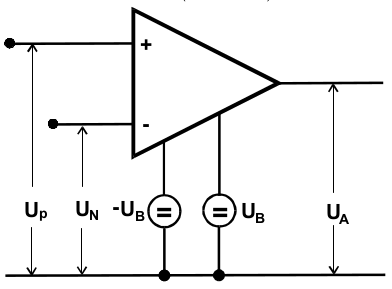
\includegraphics[width = 0.5\textwidth]{../pics/OPVBasic.png}
 \caption{Anschlüsse des Operationsverstärkers \cite{Anl}.}
 \label{pic:basic}
\end{figure}
Der mit $``+''$ gekennzeichnete Eingang wird nicht-invertierender Eingang genannt, der mit $``-''$ hingegen
invertierend. Ist das Potenzial an dem nicht-invertierenden Eingang größer als am Invertierenden,
so ist $U_A$ in Phase mit der Spannungsdifferenz $U_P-U_N$, im umgekehrten Fall gegenphasig. Die Kennlinie
des OPV ist in Abbildung \ref{pic:linie} mit übertrieben niedriger Steigung dargestellt.
\begin{figure}[t]
 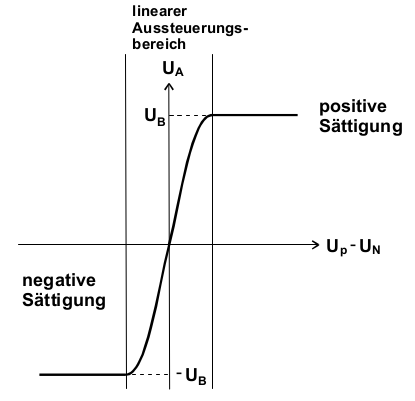
\includegraphics[width = 0.5\textwidth]{../pics/OPVLinie.png}
 \caption{Kennlinie des Operationsverstärkers \cite{Anl}.}
 \label{pic:linie}
\end{figure}
Zur Berechnung von Schaltungen mit dem OPV betrachtet man zur Vereinfachung einen idealen OPV. 
Dieser ist dadurch gekennzeichnet, dass seine Leerlaufverstärkung sowie die Eingangswiderstände unendlich hoch
sind und der Ausgangswiderstand gleich null ist. Diese Größen sind beim realen OPV natürlich
nicht mehr infitesimal. Will man Schaltungen mit OPVs genauer beschreiben,
so müssen weitere Größen betrachtet werden. Diese lauten
\begin{itemize}
 \item Gleichtaktverstärkung: Wenn $U_P = U_N$, dann ist $U_A$ dennoch ungleich null aufgrund von Asymmetrien 
 der integrierten Schaltung des OPV.
 \item Eingangsruhestrom: Dem endlichen Eingangswiderstand folgt auch ein geringer Eingangsstrom.
 \item Offsetstrom: Dies ist die Differenz der beiden Eingangsströme.
 \item Differenzeingangs- und Gleichtaktwiderstand: Mit den Eingangsruheströmen wird der Differenzeingangswiderstand
 gemessen, während eine Eingangsspannung null ist. Der Gleichtaktwiderstand ergibt sich bei gleichen Eingangsspannungen
 und der Summe der Eingangsruheströme.
 \item Offsetspannung: Hiermit wird die Asymmetrie der Eingangsspannungen beschrieben. Die Offsetspannung ist diejenige
 Spannung, welche eingestellt werden muss, damit die Ausgangsspannung gleich null ist.
 \end{itemize}
 \subsection{Linearverstärker}
 Die Sättigung beim OPV erfolgt aufgrund seiner sehr hohen Verstärkung bereits bei geringen Ansteuerungen. 
 Um die Ausgangsspannung 
 zu begrenzen und zu kontrollieren,
wird ein Teil der Ausgangsspannung an den invertierenden Eingang zurückgegeben, sodass
die Eingangsspannung verringert und somit
auch die Ausgangsspannung begrenzt wird.
Dies wird mit Gegenkopplung bezeichnet. Die
Schaltung der Linearverstärkers ist in Abbildung \ref{pic:linear}
dargestellt. 
\begin{figure}[t]
 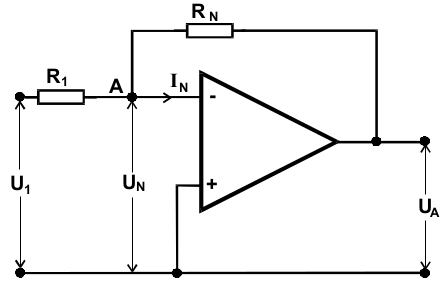
\includegraphics[width = 0.5\textwidth]{../pics/Linear.png}
 \caption{Schaltung des Linearverstärkers \cite{Anl}.}
 \label{pic:linear}
\end{figure}
Die Verstärkung lässt sich mithilfe
des idealen OPVs wie folgt berechnen. Die Eingangsspannung des idealen OPVs ist
unendlich. Daher ist der Strom $I_N$ gleich null. An dem Punkt A in Abbildung \ref{pic:linear}
addieren sich die Ströme gerade zu null. Somit gilt
\begin{align}
 0 = \frac{U_1}{R_1} + \frac{U_A}{R_N}.
\end{align}
Und die Verstärkung ergibt sich damit zu
\begin{align}
 V' = \frac{U_A}{U_1} = -\frac{R_N}{R_1}.
 \label{eq:Vprime}
\end{align}
Bei dem realen OPV bewirken die oben genannten Größen geringfügige Korrekturen.
In diesem Versuch soll nur der Einfluss der endlichen Leerlaufverstärkung betrachtet werden.
Zur Herleitung der Leerlaufverstärkung $V'$ wird der Spannungsteiler $R_1,R_N$ betrachtet.
Für diesen gilt
\begin{align}
 \frac{U_N-U_1}{U_A-U_1} = \frac{R_1}{R_1+R_N}.
\end{align}
Mit \eqref{eq:Uaus} ergibt sich die Leerlaufverstärkung zu
\begin{align}
 \frac{1}{V'} =& -\frac{U_1}{U_A} = \frac{1}{V} + \frac{R_1}{R_N}\left(1+\frac{1}{V}\right) \\
 \approx& \frac{1}{V} + \frac{R_1}{R_N}.
 \label{eq:leerlauf}
\end{align}
Für $V\gg R_N/R_1$ ergibt sich \eqref{eq:Vprime}. 
Damit zeigt sich, dass die Verstärkung 
auch für einen realen OPV nur von
dem Widerstandsverhältnis abhängt, wenn eine 
große Gegenkopplung gewählt wird. Zudem 
wird die Stabilität des Verstärkers erhöht,
da der Einfluss der Temperatur und die damit 
verbundenen Schwankungen von V nahezu
verschwinden. Die Gegenkopplung wirkt sich
zudem auf weitere Parameter des realen OPV
aus. So wird der Ausgangswiderstand verkleinert 
und die Bandbreite erhöht.

\subsection{Umkehr-Integrator}
\label{sec:int}
Die Schaltung des Umkehr-Integrators ist in
Abbildung \ref{pic:umInt} dargestellt. 
\begin{figure}[t]
 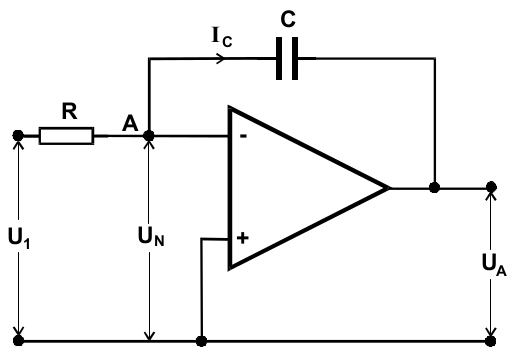
\includegraphics[width = 0.5\textwidth]{../pics/umkehrInt.png}
 \caption{Schaltung des Umkehr-Integrators \cite{Anl}.}
 \label{pic:umInt}
\end{figure}
Anstelle des Rückkopplungswiderstands ist hier ein Kondensator ein-
gebaut. Die Funktionsweise als Integrator ist
wie folgt zu sehen.
Der Strom, der über den Widerstand in den
Punkt A fließt, fließt nun auch in den Kon-
densator. Zudem wird die Ausgangsspannung
entegegen der Stromrichtung gemessen. Somit
gilt
\begin{align}
 I_C = \frac{U_1}{R} = -C \frac{\dx U_A}{\dx t}.
\end{align}
Dividieren durch $C$ und integrieren führt zu
\begin{align}
 U_A = -\frac{1}{RC} \in U_1 \dx t\,.
\end{align}
Im Falle einer Sinusspannung ist $U_A\propto \frac{1}{\omega} \cos(\omega t)$,
mit $\omega$ der Kreisfrequenz.

\subsection{Umkehr-Differenziator}
\label{sec:diff}
Die Schaltung des Differentiators ist in Abbildung \ref{pic:umDiff}
dargestellt.
\begin{figure}[t]
 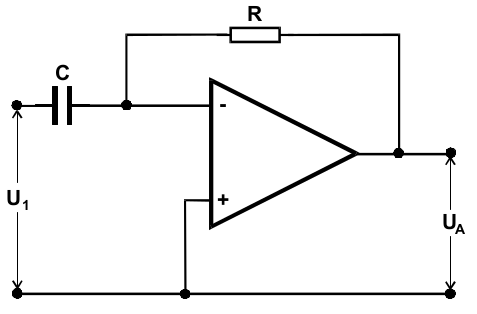
\includegraphics[width = 0.5\textwidth]{../pics/umkehrDiff.png}
 \caption{Schaltung des Umkehrdifferentiators \cite{Anl}.}
 \label{pic:umDiff}
\end{figure}
Hier sind Widerstand 
und Kondensator im Vergleich zum
Integrator vertrauscht. Die Herleitung der Wirkungsweise 
als Differentiator ist analog zu der
des Integrators. Es ergibt sich die Ausgangsspannung zu
\begin{align}
 U_A = -RC \frac{\dx U_1}{\dx t}.
\end{align}
Wieder für eine Sinusspannung gilt $U_A\propto -\omega \cos(\omega t)$.

\subsection{Schmitt-Trigger}
Der Schmitt-Trigger besitzt im Gegensatz zu
den vorherigen Schaltungen eine Mitkopplung. 
Dabei wird die Ausgangsspannung über
einen Widerstand an den nicht-invertierenden
Eingang zurückgegeben. Die Schaltung ist in
Abbildung \ref{pic:schmitt} gezeigt. 
\begin{figure}[t]
 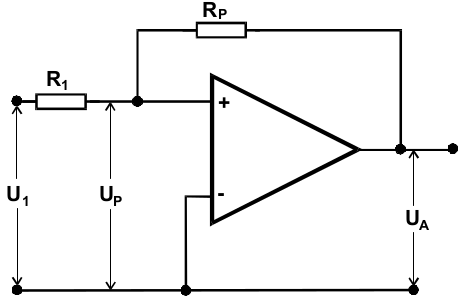
\includegraphics[width = 0.5\textwidth]{../pics/schmitt.png}
 \caption{Schaltung des Schmitt-Triggers \cite{Anl}.}
 \label{pic:schmitt}
\end{figure}
Hier wird die Eingangsspannung 
verstärkt und gleichphasig zurück auf
den Eingang gegeben. Somit wird die erhöhte
Spannung noch weiter verstärkt. Dieses Verhalten 
wird ausgenutzt, um den Schmitt-Trigger
als Schalter zu verwenden. Ist hier eine bestimmte 
Schwellspannung erreicht, so springt
die Ausgangsspannung auf die positive oder
entsprechend negative Betriebspannung. Die
Schwelle ist dabei durch
\begin{align}
 \frac{R_1}{R_P} U_B
\end{align}
gegeben und der doppelte Wert wird Schalthysterese bezeichnet.

\subsection{Signalgenerator}
Der Operationsverstärker kann ebenfalls verwendet werden, um verschiedene Formen
von Wechselspannungen zu generieren. Möglichkeiten zur Kombination der OPVs 
zu diesem Zweck sind in den Abbildungen \ref{pic:dreiRect}
und \ref{pic:sinus} dargestellt.
\begin{figure}[t]
 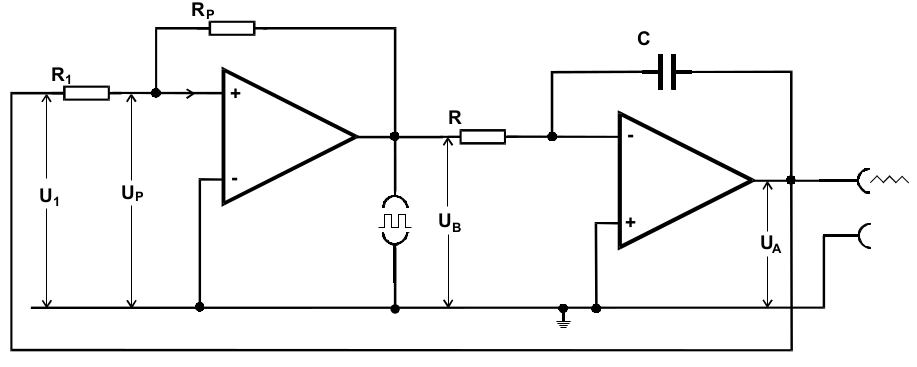
\includegraphics[width = 0.9\textwidth]{../pics/DreiRect.png}
 \caption{Schaltung des Dreiecks-/Rechteckgenerators \cite{Anl}.}
 \label{pic:dreiRect}
\end{figure}
\begin{figure}[t]
 \includegraphics[width = 0.9\textwidth]{../pics/sinus.png}
 \caption{Schaltung des Sinusgenerators \cite{Anl}.}
 \label{pic:sinus}
\end{figure}
Für einen Rechteckgenerators wird die oszillierende Rechteckspannung durch einen
Schmitt-Trigger erzeugt. Mithilfe eines Integrators kann dieses Signal 
zu einer Dreiecksspannung umgewandelt werden.\\
\noindent Die Differenzialgleichung für den gedämpften/angeregten
harmonischen Oszillator
\begin{align}
 0 = \frac{\dx^2 U_A}{\dx t}- \frac{\eta}{10 RC} \frac{\dx U_A}{\dx t} + \frac{1}{(RC)^2}U_A
\end{align}
lässt sich mit zwei hintereinander geschlossenen Integratoren und einem invertierenden
Verstärker schalten, wobei $-1<\eta<1$ mit dem Potentiometer P eingestellt wird. Die Lösung
für betragsmäßig kleine $\eta$ lautet
\begin{align}
 U_A(t) = U_0 \exp\left(\frac{\eta}{20RC}t\right) \sin\left(\frac{1}{RC}t\right).
\end{align}
Für die Schwingungsdauer ergibt sich $T=2\pi RC$ und für die Abklingdauer,
die Zeit bei der die Amplitude auf den e-ten Teil bzw. das e-fache der Amplitude geht,
gilt $\tau = 20RC/|\eta|$.

\subsection{Logarithmierer und Exponentialgenerator}
Auch wenn diese beiden Schaltungen nicht untersucht werden, soll ihre
Funktionsweise kurz geschildert werden. Die Schaltungen für den 
Logarithmierer und den Exponentialgenerator sind in den Abbildungen
\ref{pic:log} bzw. \ref{pic:exp} dargestellt.
\begin{figure}[t]
 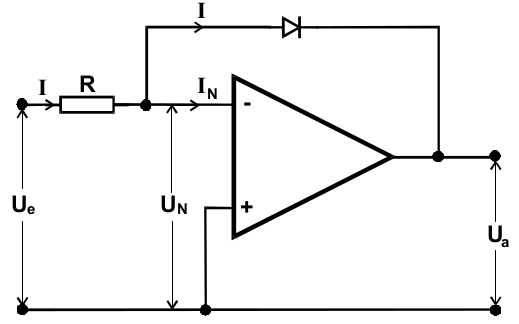
\includegraphics[width = 0.5\textwidth]{../pics/log.png}
 \caption{Schaltung des Logarithmierers \cite{Anl}.}
 \label{pic:log}
\end{figure}
\begin{figure}[t]
 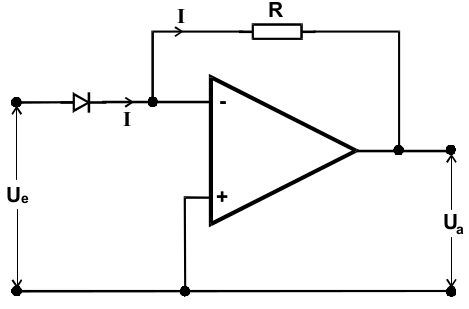
\includegraphics[width = 0.5\textwidth]{../pics/exp.png}
 \caption{Schaltung des Exponentialgenerators \cite{Anl}.}
 \label{pic:exp}
\end{figure}
Beide funktionieren unter Verwendung einer Diode. Beim Logarithmierer
befindet sich diese im Rückkopplungszweig und beim Exponentialgenerator
vor dem invertierenden Eingang. Die Diode wird verwandt, da sie eine
exponentielle Kennlinie besitzt. Im Falle eines idealen Operationsverstärkers
gelten daher
\begin{align}
 U_{A,\text{log}} = \frac{k_BT}{e_0} \ln\left(\frac{U_e}{I_0 R}\right),\\
 U_{A,\text{exp}} = RI_0\exp\left(\frac{e_0U_e}{k_BT}\right).
\end{align}



\section{Durchführung}
\subsection{Frequenzgang und Phasenbeziehung}
Die Spannungen an den beiden Eingängen am OPV sind $U_\pm = 10$\,V.
Zudem wird $R_1 = \SI{100}{\ohm}$ entsprechend Abbildung \ref{pic:linear}
gesetzt. Es soll nun $R_N$ auf vier verschiedene Werte gesetzt werden, 
um für die verschiedenen Verstärkungen $V'$ \eqref{eq:Vprime}das 
Abnehmen der Amplitude
mit steigender Frequenz $f$ festgestellt werden kann. Es soll weiterhin
darauf geachtet werden, dass die Eingangsspannung nicht höher als
\SI{100}{\milli\volt} ist. In Tabelle \ref{tab:verstaerkungen} sind
die gewählten Widerstände des Rückkopplungszweigs aufgeführt. Der
Frequenzbereich variiert zwischen $\SI{0.5}{\kilo\hertz} < f < \SI{150}{\kilo\hertz}$.
\begin{table}[b]
 \begin{tabular}{c|c}
  $R_N/\Omega$ & $V'$\\
  \hline
  500 & 5\\
  1000 & 10 \\
  3300 & 33 \\
  10000 & 100
 \end{tabular}
 \caption{Widerstände des Rückkopplungszweigs und Verstärkungen}
\label{tab:verstaerkungen}
\end{table}
Für die Phasenverschiebung zwischen Eingangs- und Ausgangsspannung
werden $R_1 = \SI{1}{\kilo\ohm}$ und $R_N = \SI{10}{\kilo\ohm}$ 
verwandt. Ihr Auftreten wird für einen Frequenzbereich 
$\SI{0.5}{\kilo\hertz} < f < \SI{100}{\kilo\hertz}$ beobachtet.

\subsection{Umkehr-Integrator und -Differenziator}
Entsprechend der Abbildungen \ref{pic:umInt} und \ref{pic:umDiff}
sollen für eine Sinus-, Dreiecks- und Rechteckspannung die Abhängigkeiten
von $U_A$ und $f=\omega/2\pi$ aus den Abschnitten \ref{sec:int} und
\ref{sec:diff} überprüft werden. Der ohmsche Widerstand ist
$R = \SI{100}{\ohm}$ und die Kapazität $C = \SI{102,3}{\nano\farad}$.
Der DC-Offset sollte so gewählt werden, dass der Gleichspannungsanteil
vom Frequenzgenerator verschwindet, damit kein konstantes Signal
mit integriert wird.

\subsection{Schmitt-Trigger}
Die Schaltung ist entsprechend Abbildung \ref{pic:schmitt} zu bauen.
Mit einer Sinusspannung am Eingang soll die Spannung ermittelt werden,
bei der die Ausgangsspannung in die Sättigungsspannung mit umgekehrten
Vorzeichen kippt. Hierfür werden $R_1 = \SI{1}{\kilo\ohm}$ und
$R_P = \SI{100}{\kilo\ohm}$ verwandt.

\subsection{Dreiecksgenerator}
Beim Dreiecksgenerator, realisiert nach Abbildung \ref{pic:dreiRect},
soll die Zeitabhängigkeit der Ausgangsspannung mit dem Oszilloskop
festgestellt und die Schwingungsfrequenz und -amplitude gemessen werden.
Die verwandten Größen sind $R_1 = \SI{1}{\kilo\ohm}$, $R_P = \SI{100}{\kilo\ohm},
R= \SI{100}{\kilo\ohm}$, $C = \SI{15}{\nano\farad}$.

\subsection{Sinusschwingungen mit zeitlich veränderlicher Amplitude}
Entsprechend dem Schaltbild \ref{pic:sinus} wird eine Sinusspannung
erzeugt mit $C_1 = \SI{21,4}{\nano\farad}$ und $C_2  = \SI{23,5}{\nano\farad}$.
Mit einem Rechteckgenerator wird am nicht-invertierenden Eingang
eine Anregung erzeugt. Die gedämpfte Schwingung $\eta = -1$ mit dem
Potentiometer am Anschlag wird mit dem Oszilloskop gespeichert und
die Frequenz im Schwingfall gemessen.



\section{Auswertung}
\subsection{Linearverstärker}
Zuerst wird die Frequenzabhängigkeit des Verstärkungsgrades betrachtet. Dazu wird die Ausgangsspannung $U_\text{A}$ eines gegengekoppelten Linearverstärkers wie in Abb. \ref{pic:linear} abhängig von Frequenz $f$ und dem Widerstand $R_\text{N}$ untersucht, weiterhin ist $R_1 = 100\ \si{\ohm}$. Zunächst wurde die Funktion $g = b \cdot x^a$ an die rechte Flanke der gemessenen Ausgangsspannung gefittet. Mit diesem wird die Grenzfrequenz $f_\text{Grenz} =\sqrt[a]{\frac{V_\text{Real}}{b\sqrt{2}}}$ bestimmt. Weiterhin wird die Leerlaufverstärkung nach Gl. \ref{eq:leerlauf} ermittelt. Schließlich ist die Frequenzabhängigkeit in Abb. \ref{pic:a plot} zu sehen.

\begin{table}
	\centering
	\caption{Gemessene und berechnete Kennwerte eines realen, gegenkoppelten Linearverstärkers}
	\begin{tabular}{lrrrr}
\hline
 $R_n$/$\Omega$                           & 1000      & 500      & 10000      & 330      \\
 $a$                                      &   -0.38   &  -0.16   &    -0.91   &  -0.13   \\
 $\Delta a$                               &    0.0016 &   0.0004 &     0.0002 &   0.0001 \\
 $b$/V                                    &    1.77   &   0.37   &    32.83   &   0.25   \\
 $\Delta b$/V                             &    0.101  &   0.001  &     3.267  &   0      \\
 $V_\text{Real}$                          &    0.44   &   0.21   &     4.36   &   0.15   \\
 $f_\text{Grenz}$/kHz                     &   98.59   & 352.48   &    13.51   & 661.94   \\
 $\Delta f_\text{Grenz}$/kHz              &   14.84   &   8.2    &     1.48   &   5.33   \\
 $V_\text{Real} \cdot f_\text{Grenz}$/kHz &   43.14   &  73.11   &    58.93   &  98.12   \\
 $V_\text{Leerlauf}$                      &    2.19   &   4.62   &     0.22   &   6.44   \\
\hline
\end{tabular}
	\label{table:a_real}
\end{table}

\begin{table}
	\centering
	\begin{tabular}{lll}
\hline
 $R_n$ [$\Omega$] & $R_1$ [$\Omega$] & $V_\text{Theorie}$ \\
 1000             & 100              & 10.0               \\
 500              & 100              & 5.0                \\
 10000            & 100              & 100.0              \\
 330              & 100              & 3.3                \\
\hline
\end{tabular}
	\caption{Theoretische Verstärkung eines idealen, gegengekoppelten Linearverstärkers}
	\label{table:a_theorie}
\end{table}

\begin{figure}
	\centering
	\includegraphics[width=\textwidth]{../auswertung/results/a/a.pdf}
	\caption{Frequenzabhägigkeit des Verstärkungsgrades eines gegengekoppelten Linearverstärkers mit $U_1 = 20$ V}
	\label{pic:a plot}
\end{figure}

\subsection{Umkehrintegrator}
Es wird eine Schaltung wie in Abb. \ref{pic:umInt} verwandt, um einen Umkehr-Integrator mit $R = 100\ \si{\ohm}$ und $C = 102.3\ \si{\nano\farad}$ zu realisieren. Als Eingangsspannungen werden nacheinander Sinus-,Rechteck- und Dreieckspannung angelegt. Am Ausgang sind dann die integrierten Spannungen zu messen, s. Abbildungen \ref{pic:b sinus},\ref{pic:b rechteck},\ref{pic:b dreieck}. Zur besseren Sichtbarkeit wurde die Amplitude des Eingangs- und Ausgangssignals normiert.

\begin{figure}
	\centering
	\includegraphics[width=0.7\textwidth]{../auswertung/results/b/sinus.pdf}
	\caption{Gemessene Eingangs- und Ausgangspannung eines Umkehrintegrators mit angelegter Sinusspannung, $f = 0.1\ \si{\kilo\hertz}$}
	\label{pic:b sinus}
\end{figure}

\begin{figure}
	\centering
	\includegraphics[width=0.7\textwidth]{../auswertung/results/b/rechteck.pdf}
	\caption{Gemessene Eingangs- und Ausgangspannung eines Umkehrintegrators mit angelegter Rechteckspannung, $f = 0.1\ \si{\kilo\hertz}$}
	\label{pic:b rechteck}
\end{figure}

\begin{figure}
	\centering
	\includegraphics[width=0.7\textwidth]{../auswertung/results/b/dreieck.pdf}
	\caption{Gemessene Eingangs- und Ausgangspannung eines Umkehrintegrators mit angelegter Dreieckspannung, $f = 0.1\ \si{\kilo\hertz}$}
	\label{pic:b dreieck}
\end{figure}

Weiterhin wird die charakteristische Kurve der Schaltung aufgenommen. Dazu wird die Ausgangspannung gegen den Kehrwert der Frequenz aufgetragen. Für den Fit wurde die Funktion $g = b \cdot x^a$ verwandt, das Ergebnis ist in Abb. \ref{pic:b charKurve} zu sehen.

\begin{figure}
	\centering
	\includegraphics[width=0.7\textwidth]{../auswertung/results/b/charKurve.pdf}
	\caption{Charakteristische Kurve des Umkehrintegrators mit angelegter Sinusspannung,\protecta = (-0.38 $\pm$ 6.3$\cdot 10^{-6}$), \protect$b = (9.32\pm9.28e-06)\ \si{\volt}$ }
	\label{pic:b charKurve}
\end{figure}

\subsection{Umkehrdifferentiator}
An dieser Stelle wird eine Schaltung wie in Abb. \ref{pic:umDiff} verwandt. Es wurden die gleiche Kapazität und der gleiche Widerstand wie beim Umkehrintegrator verwandt.

\begin{figure}
	\centering
	\includegraphics[width=0.7\textwidth]{../auswertung/results/c/sinus.pdf}
	\caption{Gemessene Eingangs- und Ausgangspannung eines Umkehrdifferentiators mit angelegter Sinusspannung, $f = 0.1\ \si{\kilo\hertz}$}
	\label{pic:c sinus}
\end{figure}

\begin{figure}
	\centering
	\includegraphics[width=0.7\textwidth]{../auswertung/results/c/rechteck.pdf}
	\caption{Gemessene Eingangs- und Ausgangspannung eines Umkehrdifferentiators mit angelegter Rechteckspannung, $f = 0.1\ \si{\kilo\hertz}$}
	\label{pic:c rechteck}
\end{figure}

\begin{figure}
	\centering
	\includegraphics[width=0.7\textwidth]{../auswertung/results/c/dreieck.pdf}
	\caption{Gemessene Eingangs- und Ausgangspannung eines Umkehrdifferentiators mit angelegter Dreieckspannung, $f = 0.1\ \si{\kilo\hertz}$}
	\label{pic:c dreieck}
\end{figure}

Auch hier wird eine charakteristische Kurve erstellt. Die Ergebnisse sind in Abb. \ref{pic:c charKurve} und Tab. \ref{table:c fitParameter} zu sehen.

\begin{figure}
	\centering
	\includegraphics[width=0.7\textwidth]{../auswertung/results/c/charKurve.pdf}
	\caption{Charakteristische Kurven des Umkehrdifferentiators bei verschiedenen angelegten Spannungen}
	\label{pic:c charKurve}
\end{figure}

\begin{table}
	\centering
	\begin{tabular}{lll}
\hline
 Spannungsfunktion & $a$                    & $b\ [\si{\volt}]$                 \\
 Sinus             & $(-1.01\pm0.00019891)$ & $(5.69\pm0.00236534)\ \si{\volt}$ \\
 Dreieck           & $(-0.99\pm1.802e-05)$  & $(7.95\pm0.0004173)\ \si{\volt}$  \\
 Rechteck          & $(-0.0\pm5.5e-07)$     & $(17.5\pm0.0001564)\ \si{\volt}$  \\
\hline
\end{tabular}
	\caption{Ermittelte Fitparameter der charakteristischen Kurve für verschiedene Spannungsfunktionen angelegt an den Umkehrdifferentiator}
	\label{table:c fitParameter}
\end{table}

\subsection{Schmitt-Trigger}
Für die Schaltung nach Abb. \ref{pic:schmitt} wurden $R_1 = 1 \si{\kilo\ohm}$ und $R_p = 100 \si{\kilo\ohm}$ verwandt. Als Kippspannung wurde $U_\text{Kipp} = 0.182\ \si{\ohm}$ bestimmt.

\subsection{Dreickeckgenerator}
Die Schaltung wurde wie in Abb. \ref{pic:dreiRect} ausgeführt und es wurden die folgenden Bauteile verwandt: $R_1 = 1\ \si{\kilo\ohm}$, $R_p = 100\ \si{\kilo\ohm}$, $R = 100\ \si{\kilo\ohm}$ und $C$ = 15 nF. Die gemessenen Frequenzen betragen $f_\text{Rechteck} = 5.98\ \si{\kilo\hertz}$ und $f_\text{Dreieck} = 6.00\ \si{\kilo\hertz}$, sowie $U_\text{Rechteck} = 17.9\ \si{\volt}$ und $U_\text{Dreieck} = 0.44\ \si{\volt}$.

\subsection{Phasenverschiebung}
Mithilfe einer Schaltung wie in Abb. \ref{pic:linear} wird die Frequenzabhängigkeit der Phase zwischen Eingang und Ausgangs untersucht. Dazu wird ein Fit mit $g = A \cdot \cos (\omega t + \phi)$ an sowohl Eingangs- als auch Ausgangssignal durchgeführt. Die resultierende Phase ist dann $\Delta \varphi = \varphi_\text{Ein} - \varphi_\text{Aus}$. Diese wird gegen die Frequenz aufgetragen, in Abb. \ref{pic:e phase} zu sehen.

\begin{figure}
	\centering
	\includegraphics[width=0.7\textwidth]{../auswertung/results/e/phase.pdf}
	\caption{Frequenzabhängiges Phasenverhalten eines gegengekoppelten Linearverstärkers}
	\label{pic:e phase}
\end{figure}

\section{Diskussion}
Besonders bei der Betrachtung des gegengekoppelten Linearvertärkers wird klar, wie weit der reale Operationsverstärker vom idealen entfernt ist. Die real gemessenen Verstärkungsgrade liegen weit unter den theoretisch möglichen, was unter anderem an der hohen Leerlaufverstärkung liegen könnte. Außerdem bewegt sich die Bandbreite innerhalb einer Größenordnung, was vielleicht an den sehr unterschiedlichen, eingesetzten Widerständen liegen kann.

Sowohl Umkehrintegrator, als auch -differentiator haben sich in den untersuchten Bereichen wie erwartet verhalten. Beide verhielten sich $\propto f^{-1}$, was zu erwarten war, ausgenommen nur die Rechteckspannung am Differentiator, da die resultierenden Delta-Peaks die gleiche Höhe wie das Eingangssignal aufwiesen.

\newpage
 \begin{thebibliography}{WissOnl}
 	\bibitem{Anl} TU Dortmund Anleitung für Versuch Nr.51 \url{http://129.217.224.2/HOMEPAGE/Anleitung_FPBSc.html}
 	\end{thebibliography}

% ========================================
%	Literaturverzeichnis
% ========================================

%\bibliographystyle{plainnat}			% Bibliographie-Style auswählen
%\bibliography{BIBDATEI}			% Literaturverzeichnis

% ========================================
%	Das Dokument endent
% ========================================
\end{document}
